%%%%%%%%%%%%%%%%%%%%%%%%%%%%%%%%%%%%%%%%%%%%%%%%%%
% Basic setup. Most papers should leave these options alone.
\documentclass[fleqn,usenatbib]{mnras}

% MNRAS is set in Times font. If you don't have this installed (most LaTeX
% installations will be fine) or prefer the old Computer Modern fonts, comment
% out the following line
\usepackage{newtxtext,newtxmath}
% Depending on your LaTeX fonts installation, you might get better results with one of these:
%\usepackage{mathptmx}
%\usepackage{txfonts}

% Use vector fonts, so it zooms properly in on-screen viewing software
% Don't change these lines unless you know what you are doing
\usepackage[T1]{fontenc}

% Allow "Thomas van Noord" and "Simon de Laguarde" and alike to be sorted by "N" and "L" etc. in the bibliography.
% Write the name in the bibliography as "\VAN{Noord}{Van}{van} Noord, Thomas"
\DeclareRobustCommand{\VAN}[3]{#2}
\let\VANthebibliography\thebibliography
\def\thebibliography{\DeclareRobustCommand{\VAN}[3]{##3}\VANthebibliography}


%%%%% AUTHORS - PLACE YOUR OWN PACKAGES HERE %%%%%

% Only include extra packages if you really need them. Common packages are:
\usepackage{graphicx}	% Including figure files
\usepackage{amsmath}	% Advanced maths commands
\usepackage{amssymb}	% Extra maths symbols

%%%%%%%%%%%%%%%%%%%%%%%%%%%%%%%%%%%%%%%%%%%%%%%%%%

%%%%% AUTHORS - PLACE YOUR OWN COMMANDS HERE %%%%%

% Please keep new commands to a minimum, and use \newcommand not \def to avoid
% overwriting existing commands. Example:
%\newcommand{\pcm}{\,cm$^{-2}$}	% per cm-squared

%%%%%%%%%%%%%%%%%%%%%%%%%%%%%%%%%%%%%%%%%%%%%%%%%%

%%%%%%%%%%%%%%%%%%% TITLE PAGE %%%%%%%%%%%%%%%%%%%

% Title of the paper, and the short title which is used in the headers.
% Keep the title short and informative.
\title[Hot Accretion in FIRE]{Galactic Discs Fed by Hot Accretion in FIRE}

% The list of authors, and the short list which is used in the headers.
% If you need two or more lines of authors, add an extra line using \newauthor
\author[\ldots]{
\ldots,$^{1}$\thanks{E-mail: mn@ras.org.uk (KTS)}
\\
% List of institutions
$^1$ \ldots
}

% These dates will be filled out by the publisher
\date{Accepted XXX. Received YYY; in original form ZZZ}

% Enter the current year, for the copyright statements etc.
\pubyear{2020}

% Don't change these lines

\newcommand{\Rcool}{R_{T=10^5\,{\rm K}}}
\newcommand{\tcon}{t_{T=10^5\,{\rm K}}}
\newcommand{\Mdot}{\dot{M}}
\newcommand{\Rcirc}{R_{\rm circ}} %need better name as R_cool means something else
\newcommand{\Rvir}{R_{\rm vir}}

\begin{document}
\label{firstpage}
\pagerange{\pageref{firstpage}--\pageref{lastpage}}
\maketitle

% Abstract of the paper
\begin{abstract}

We study how gas accretes onto $\sim L^\star$ star-forming galaxies at redshift $z\sim0$ using the FIRE cosmological simulations. We evaluate the relative importance of three modes of accretion: gas that never heats to the virial temperature (`cold accretion'), hot gas that condenses into cool clouds in the halo which then accretes onto the galaxy (``condensation''), and gas that remains hot down to the galaxy scale (`cooling flow'). 
We demonstrate that across our sample of four MW-mass halos the primary mode of gas accretion is `cooling flow', with an inflow rate $\sim xx\times$ that of other accretion modes. Gas accreted in this mode is hot and spherical down to  $\lesssim 0.1 \Rvir$ where $\Rvir$ is the halo virial radius, at which point it simulationously cools and circularizes thus joining the outskirts of the galactic disc. 
Accretion via condensation is subsdominant, and mainly associated with satellites galaxies (?). Cold accretion does not occur in significant quantities in our sample. 
% Using particle tracking we demonstrate that gas remains hot until it cools when it circularizes at 
% \textit{Gas cools after circularizing because it is no longer undergoing compressional heating that offsets cooling.}
% \textbf{Check the numbers.}
\end{abstract}

% Select between one and six entries from the list of approved keywords.
% Don't make up new ones.
\begin{keywords}
keyword1 -- keyword2 -- keyword3
\end{keywords}

%%%%%%%%%%%%%%%%%%%%%%%%%%%%%%%%%%%%%%%%%%%%%%%%%%

%%%%%%%%%%%%%%%%% BODY OF PAPER %%%%%%%%%%%%%%%%%%

\subsection{ KEY FOR COAUTHORS}
\textbf{Bold: Notes for things to implement.} \\
\textit{Italics: Rough text, needs polishing.} \\
Normal: Normal text, polished enough to be included in a draft.

\section{Introduction}

% Accretion in cosmological simulations
\textbf{Ho,Martin+2019}

% Modes of hot accretion
\textit{
Two modes of hot accretion:
\begin{itemize}
    \item condensation (Maller \& Bullock 2004; Kaufmann, Bullock+09; McCourt+12; Voit+17)
    \item classic CF (Cowie+80; Paper I)
\end{itemize}
}
\textbf{Intro TBD}

\section{Methods}

% Simulation sample
\textit{
We use four simulations:
m12i\_md\_7100, m12b\_md\_7100, m12f\_core\_7100, m12m\_core\_7100
}
\textbf{Also do massive galaxies?}
\textbf{Do more metal diffusion simulations (the non-md sims have unexpected cooling at large radii): at least 4 metal diffusion simulations would be good.}

% How we select the particles
\textit{
For a given galaxy we select all particles that are in the central galaxy at $z=0$ and in the CGM 1 Gyr prior.
The galaxy is defined as all gas and stars inside $R_{\rm gal} = 0.1 R_{\rm vir}$, with an additional density cut of $n_{\rm H} = 0.13$ cm$^{-3}$ for gas.
The CGM is defined as all gas inside $0.1 -1 R_{\rm vir}$.
For each selected particle we retrieve the full history of the particle (including temperature, density, metallicity) throughout the simulation.
}

\textbf{The number of IDs that are accreted for m12i is 18554.
However, after removing duplicates, the number of IDs that are tracked is 14703.
Either $\sim20\%$ of the particles split, or this is a symptom of a bug.
Find out which.}

% Definition of t1e5 and calculating it
\textit{
$\tcon$ is the latest time among our particles at which the particle transitions from $T > 10^5$ K to $T< 10^5$ K.
(When selecting values in the simulation corresponding to $\tcon$ we use the last snapshot an accreted particle had $T > 10^5$ K, i.e. the snapshot immediately before the transition.)
Note that we do not account for gas particles being heated to $T > 10^5$ K while still in the ISM.
Because our sample of tracked particles focuses on recently accreted particles this is expected to be a small population that will not contaminate our analysis.
This is confirmed after-the-fact in Figure~\ref{f: theta vs R}, where gas is not preferentially oriented in a disky ISM prior to $\tcon$.
}
\textbf{We could select out ISM-heated particles, if necessary, but as noted above Figure~\ref{f: theta vs R} shows that this is not an issue.}

\begin{equation}
    \Rcool \equiv R(t_{T=10^5\,{\rm K}})
\end{equation}


\textit{the circularization radius $\Rcirc$ is defined via}
\begin{equation}
    j = v_{\rm c}(\Rcirc)\Rcirc
\end{equation}
\textit{where $j$ is the specific angular momentum and $v_{\rm c}$ is the circular velocity.}

\textbf{When calculating the cooling function I just used Y=0.2485. That should be fine, right?}

\section{Results}

\begin{figure}
    \centering
    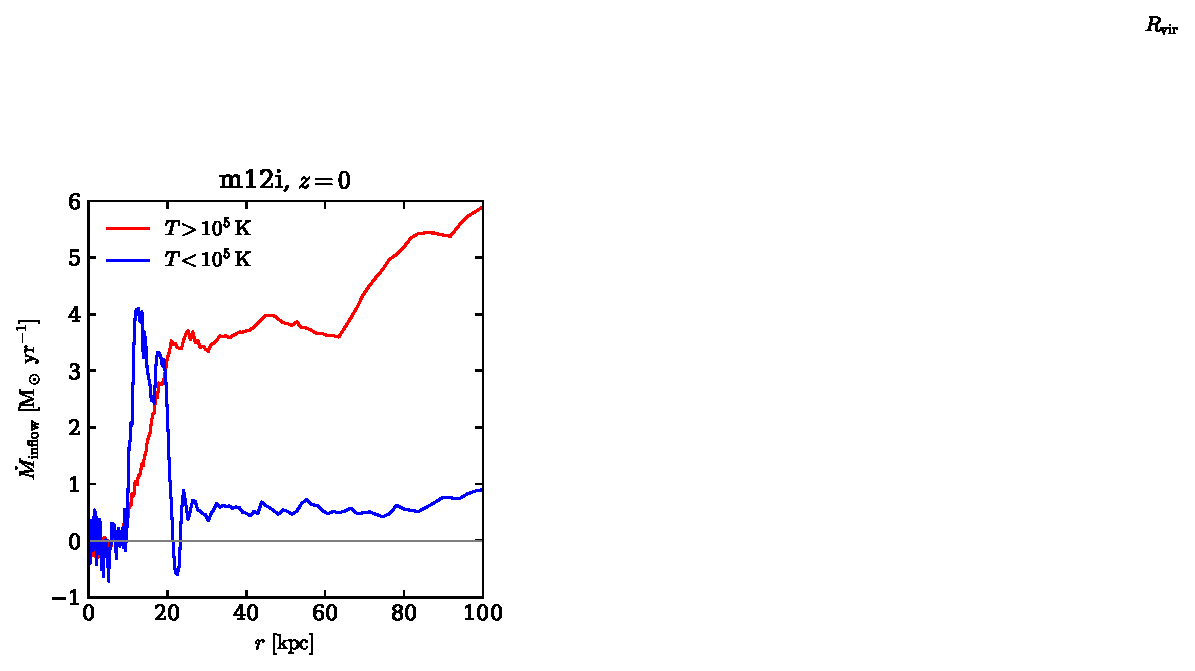
\includegraphics{Mdot_m12i.pdf}
    \caption{
    Mass inflow in spherical shells as a function of radius for $T < 10^5$ K gas (blue) and $T>10^5$ K (red) gas.
    Most inflowing gas at $r\gtrsim 20 $ kpc is hot.
    \textbf{Add images of face-on $z=0$ slice with temperature and velocity arrows.}
    \textbf{Add SFR$(>r)$}
    % \textbf{Add cuts on density/temperature to avoid ISM gas causing a wide dispersion at low-r.}
    % \textbf{Change to linear space to emphasize halo. Cut out accretion shock.}
    }
    \label{f:Mdot}
\end{figure}

\begin{figure}
    \centering
    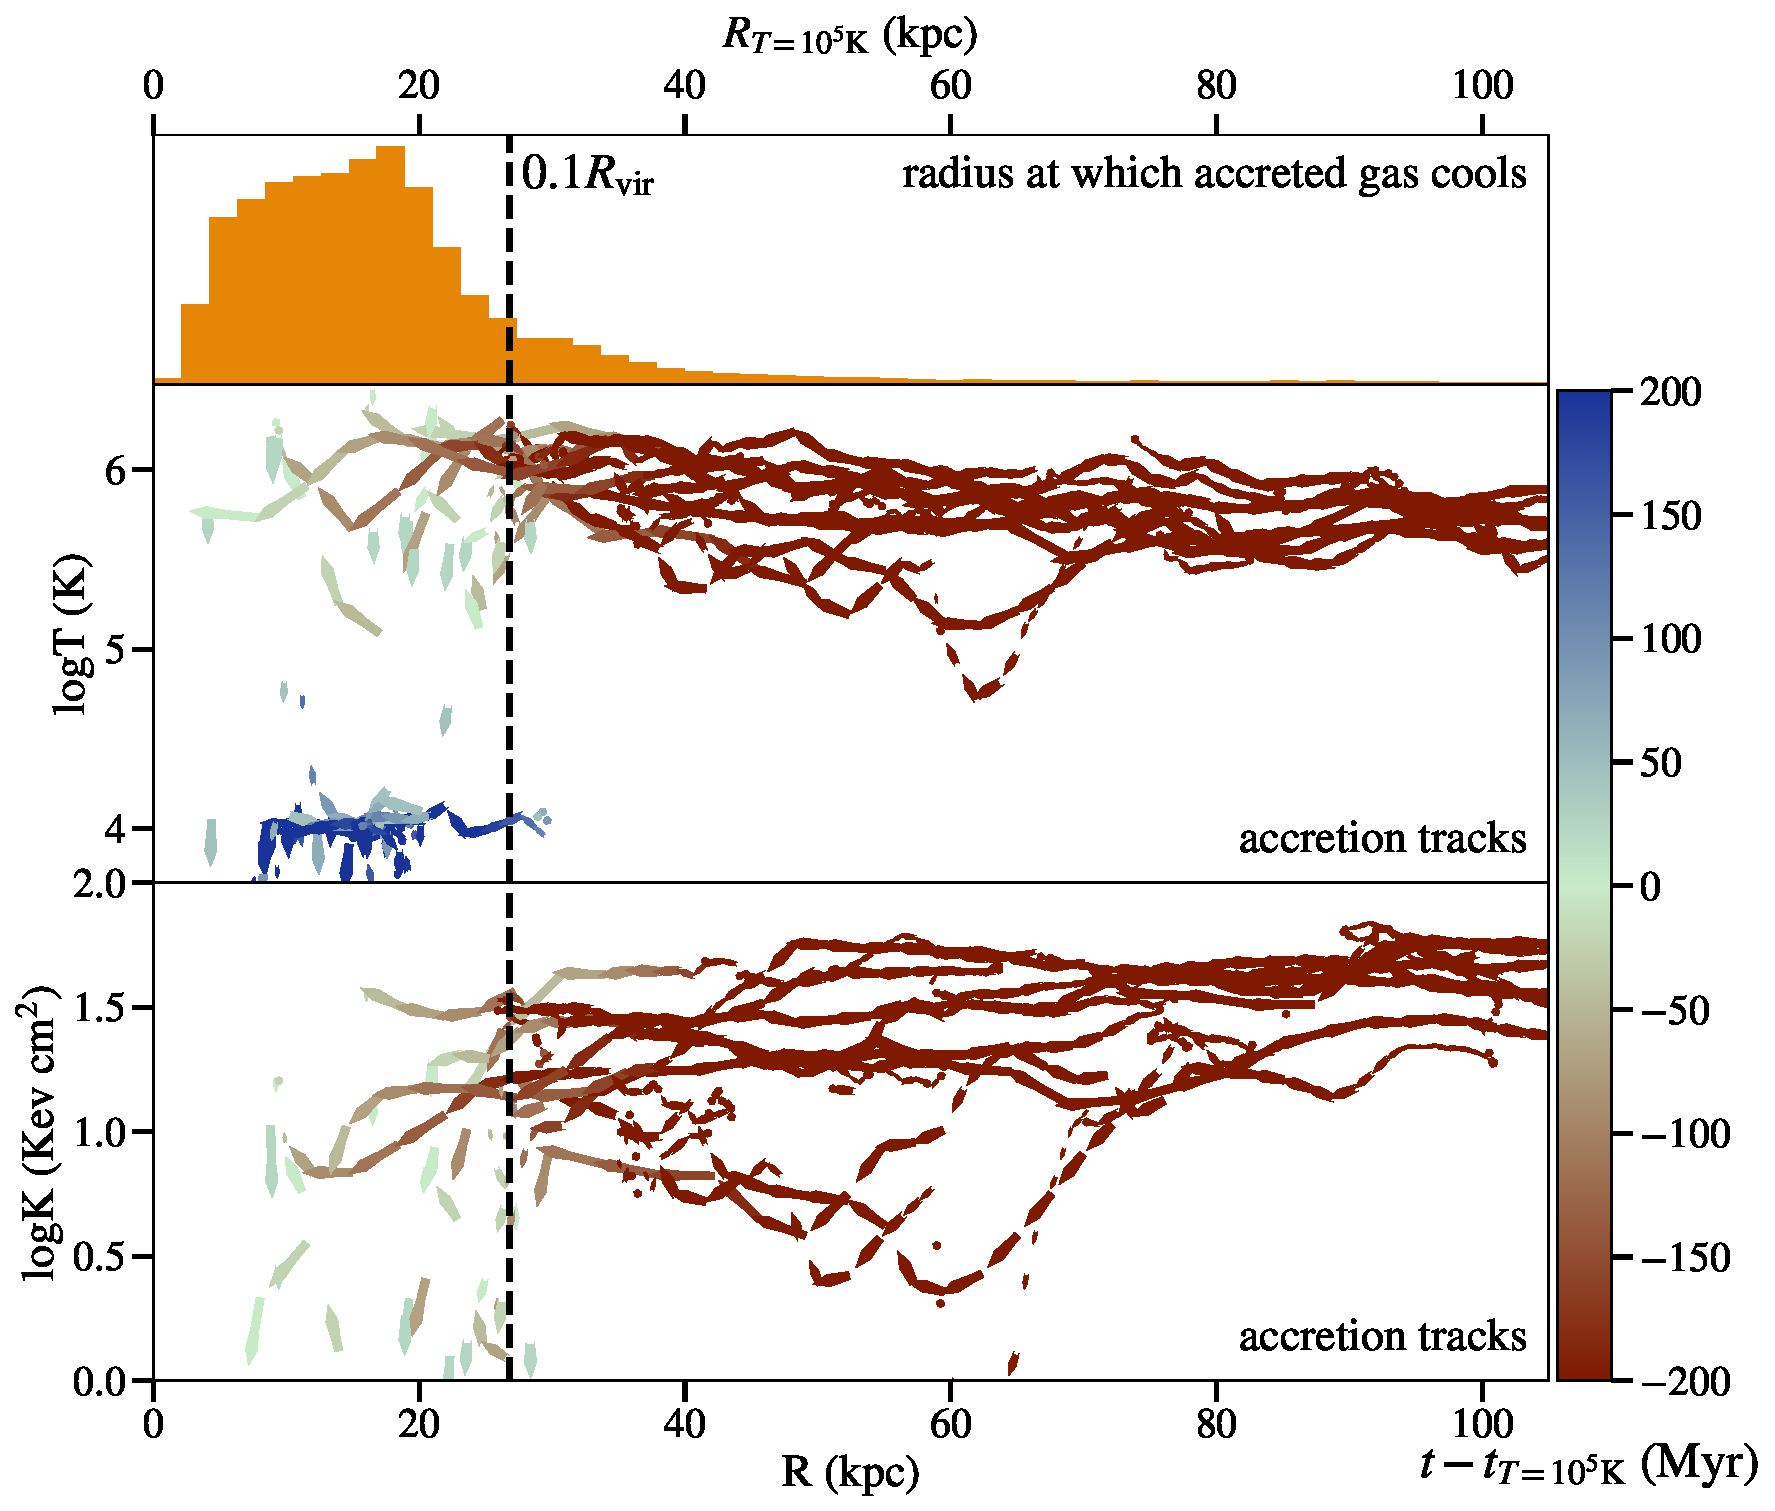
\includegraphics[width=\columnwidth]{figures/tracks_m12i_md.pdf}
    \caption{
    \textbf{Main panel:} 10 T vs.\ R and K vs.\ R tracks for an $L^\star$ halo at $z=0$ (\texttt{m12i\_md}), with color indicating time minus accretion time.
    Gas remains hot until cooling at $\lesssim 0.1 R_{\rm vir}$.
    \textbf{Top panel:} Distribution of $\Rcool$, the radius at which gas particles last transitioned from $T > 10^5$ K to $T < 10^5$ K prior to accreting, i.e. the radius at which they cooled prior to accretion.
    }
    \label{f: T vs R}
\end{figure}

\begin{figure}
    \centering
    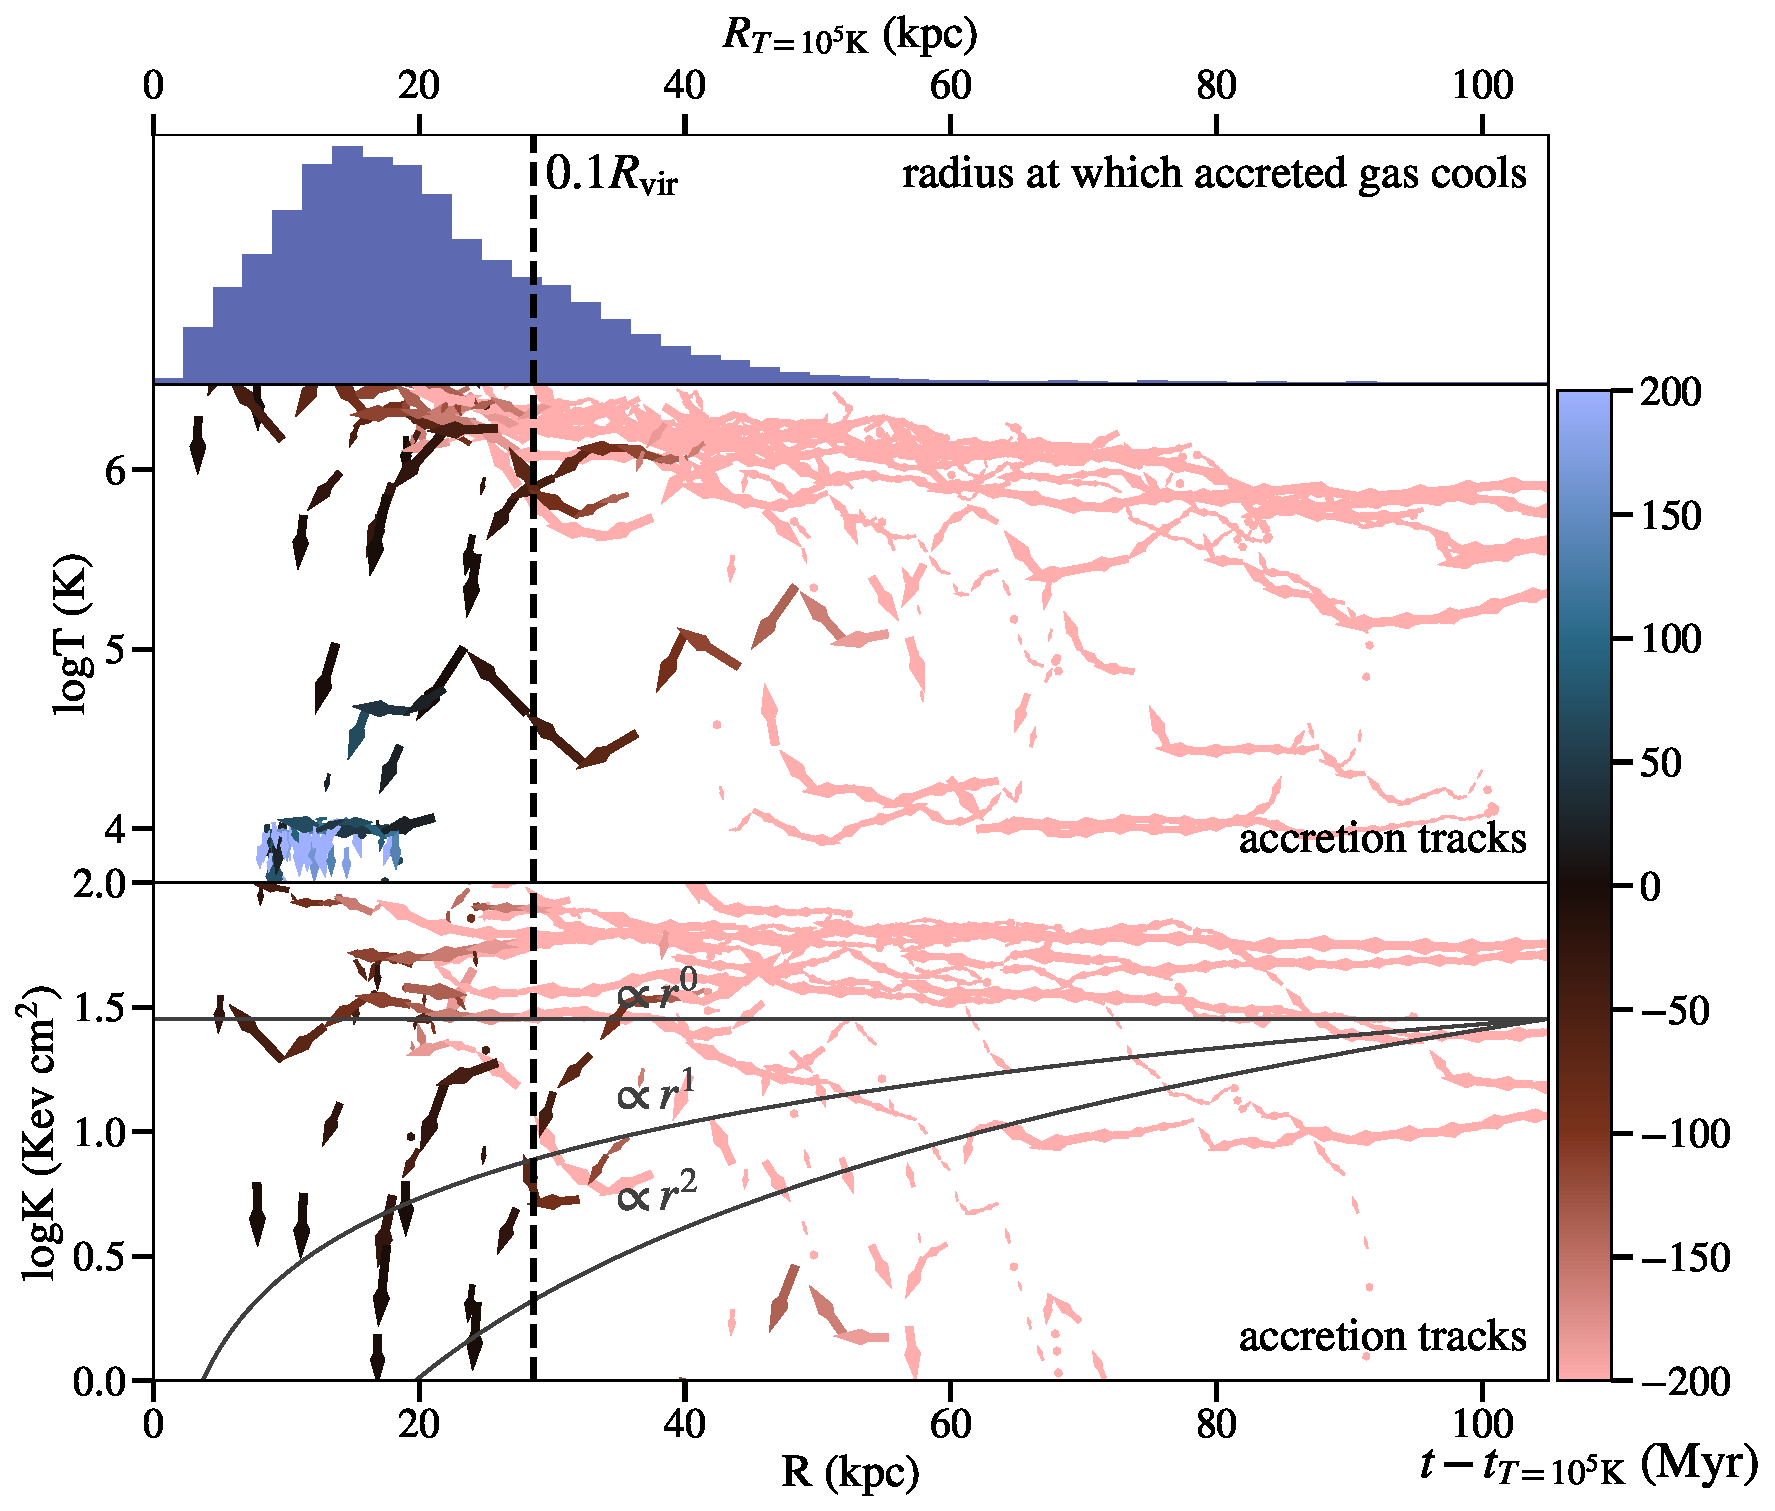
\includegraphics[width=\columnwidth]{figures/tracks_m12b_md.pdf}
    \caption{
    Same as Figure~\ref{f: T vs R}, but for \texttt{m12b\_md}.
    }
    \label{f: T vs R m12b_md}
\end{figure}

% \begin{figure}
% \centering
% 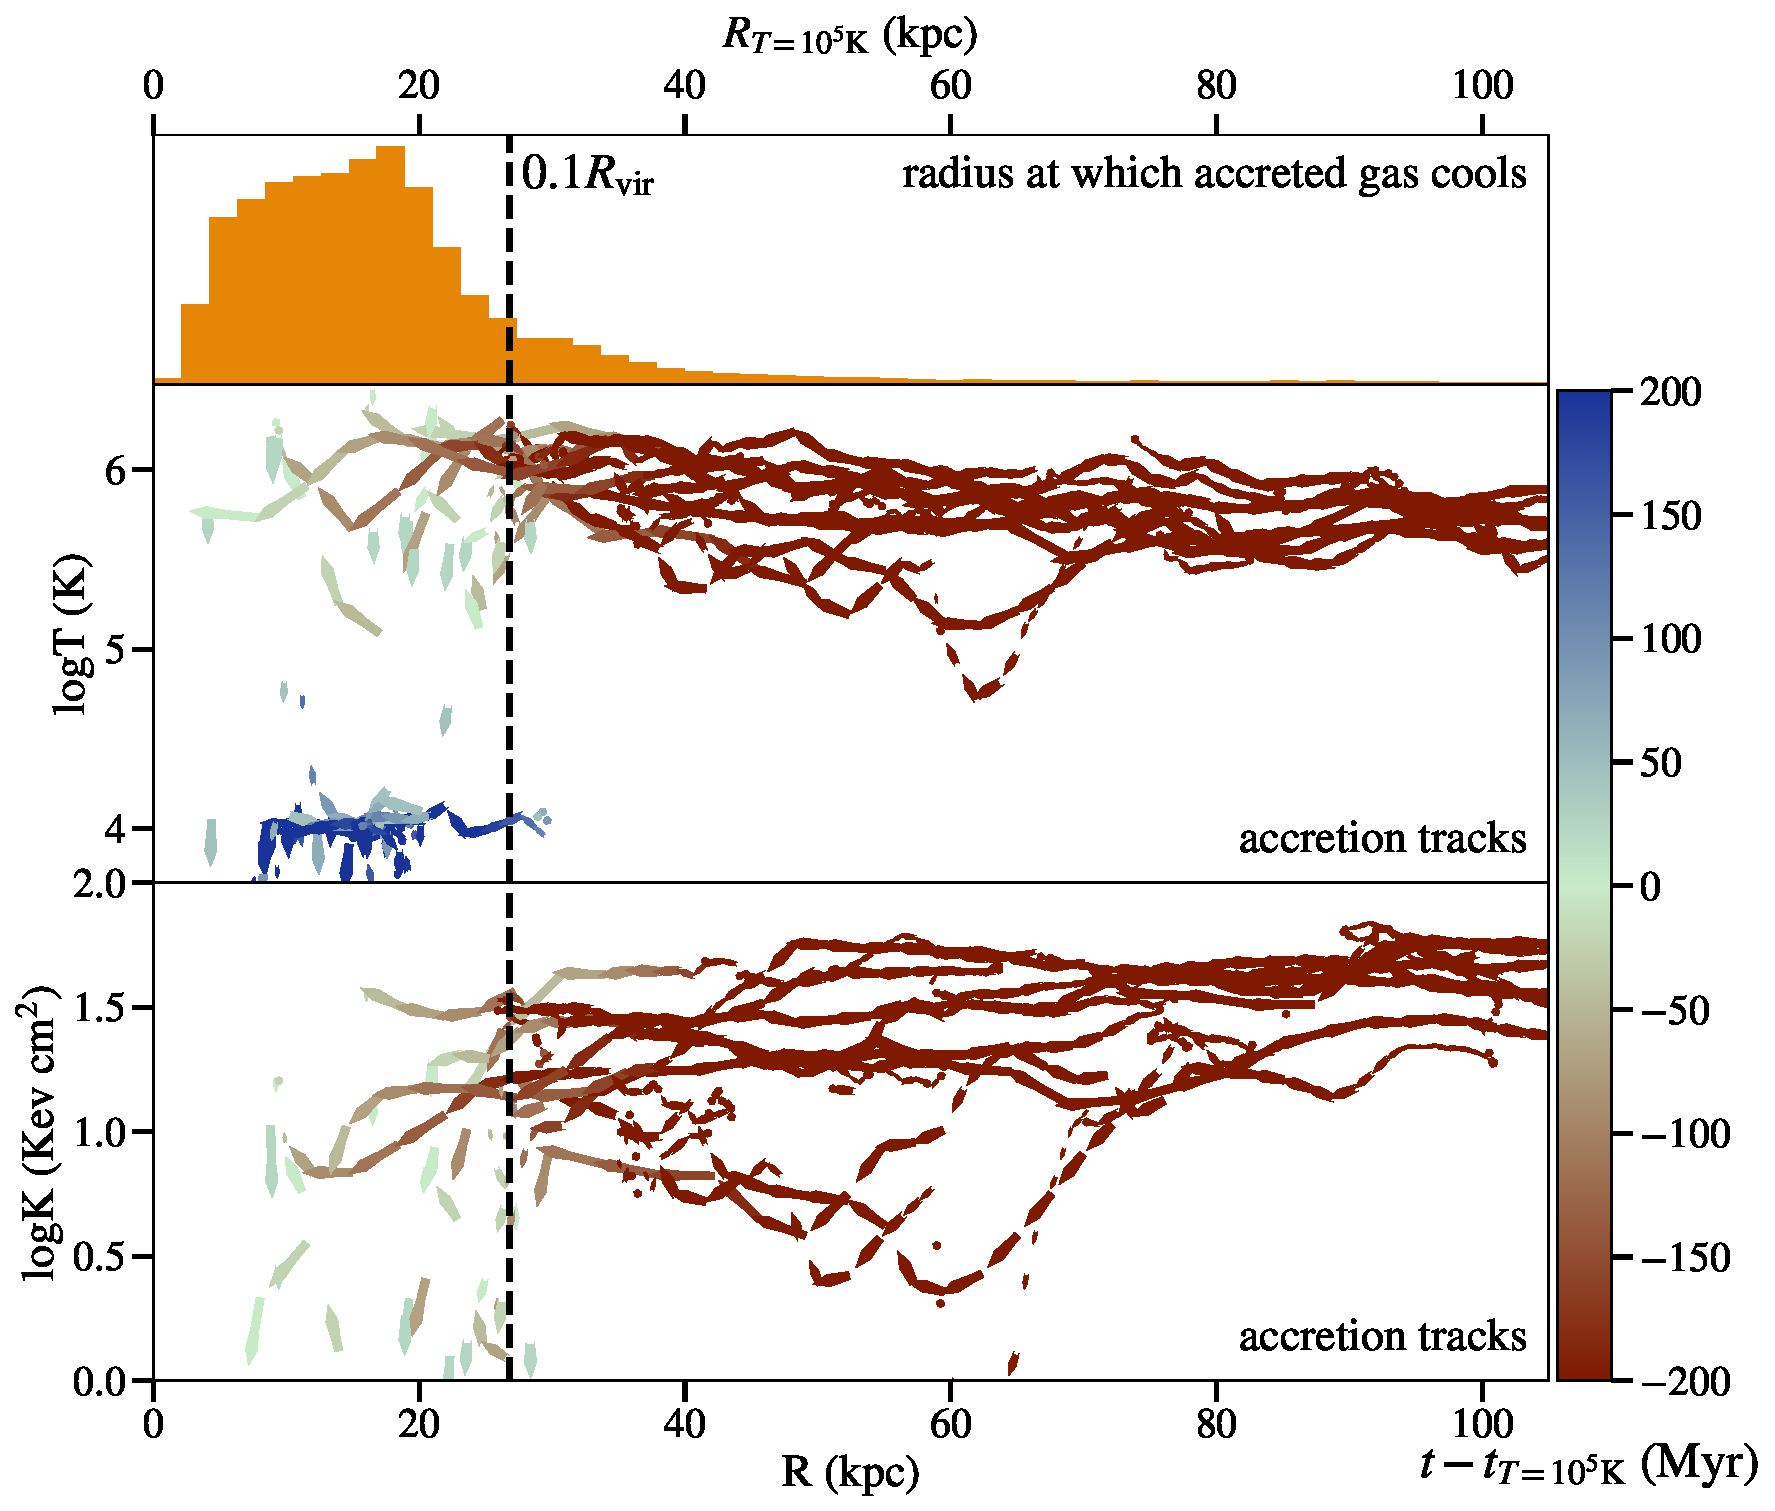
\includegraphics[width=\columnwidth]{figures/tracks_m12i_md.pdf}
% \end{figure}

\begin{figure}
    \centering
    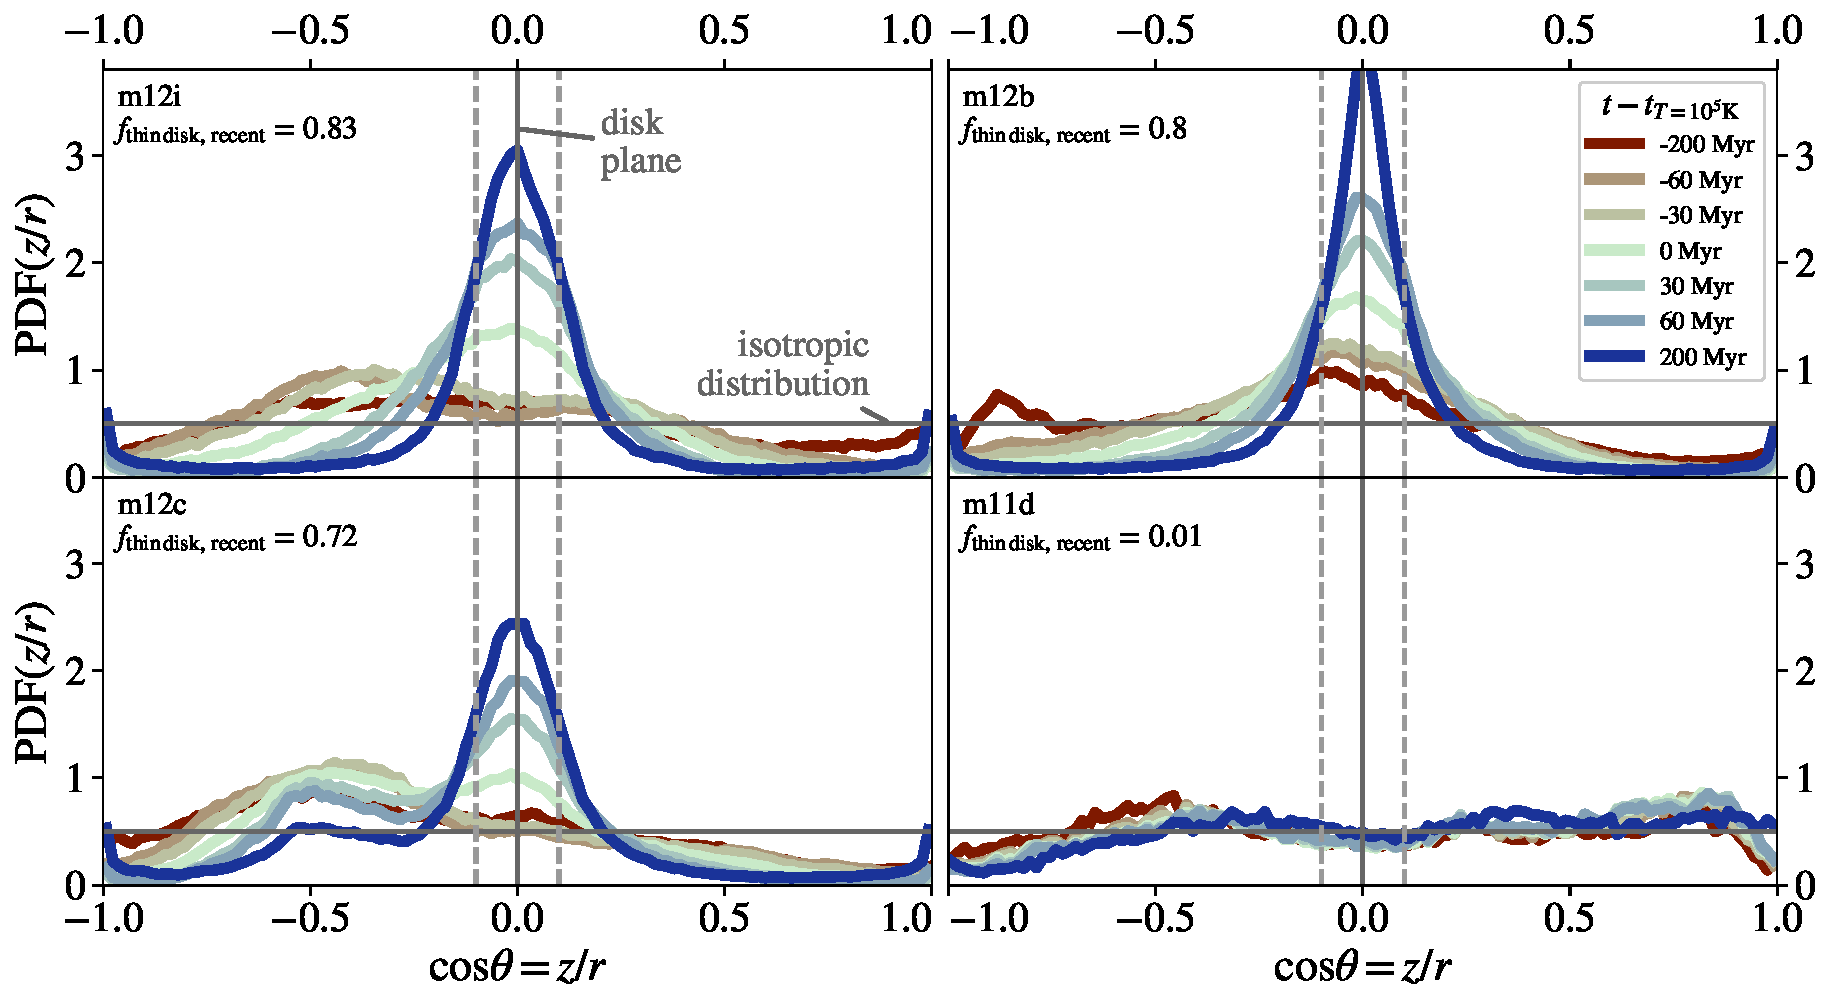
\includegraphics[width=\columnwidth]{figures/theta_vs_t.pdf}
    \caption{
    Angular distribution of accreting gas over 250 Myr before/after cooling.
    Prior to cooling the gas is distributed without a strong preferential direction (as shown by the consistency with the horizontal line representing a spherical PDF).
    After cooling the gas is primarily found in the disk at $\cos\ \theta = 0$.
    }
    \label{f: theta vs R}
\end{figure}

\begin{figure*}
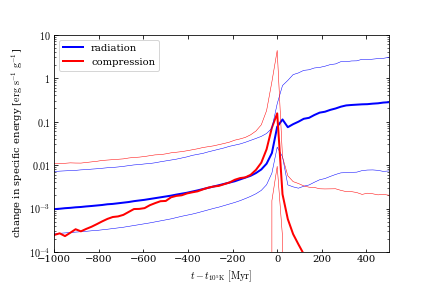
\includegraphics[width=\columnwidth]{rad_vs_compress.png}
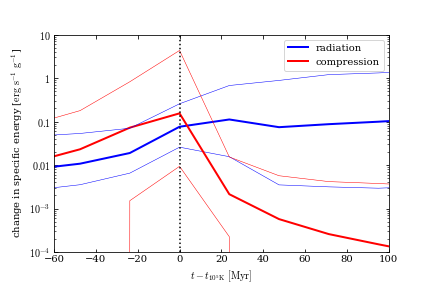
\includegraphics[width=\columnwidth]{rad_vs_compress_zoom.png}
\caption{
Compressional heating rate vs cooling rate of accreted particles as a function of time relative to $t(T=10^5\,{\rm K})$.
Thick lines are medians while thin lines are 16 and 84 percentiles.
Right panels focuses on $-60 - 100$ Myr.
This figure shows that gas cools when the cooling is no longer offset by compressive heating.
\textbf{
Add a vertical line in the left panel at t-t1e5=0.
}
\textbf{
Make labels bigger, and space between figures smaller.
}
\textbf{
Change image type to PDF so it never loses resolution.
}
\textbf{
Consider adding an individual track or a few on top (will definitely need to make the lines into shaded regions if we do this).
}
}
\end{figure*}

\begin{figure}
    \centering
    % \includegraphics{}
    \caption{
    \textbf{Spare figure, but maybe
    cooling emission in X-ray, optical and UV lines vs.\ radius, only from tracked particles
    }
    }
    \label{f:emission}
\end{figure}

% Accretion tracks figure description
\textit{
The main panels of Figure~\ref{f: T vs R} show the paths in temperature-radius and entropy-radius space taken by accreting particles.
}

% Distribution of r1e5
\textit{
As an explicit example of how far our distribution is from a condensation model, isotropic cooling occurring randomly within $R_{\rm vir}$ would cool in a wide distribution with a median at $0.8 R_{\rm vir}$, while for our accreted gas the median $\Rcool \approx 0.06 R_{\rm vir}$.
}
\textit{We added all particles with $\Rcool>100$ to $R=100$ bin, so we don't ignore them.}

\section{Discussion}

\subsection{AGN feedback}

\textit{
\begin{itemize}
    \item Results expected to be valid after disc forms (Paper III) and before AGN feedback kicks in (ref.~Byrne+)
    \item Results are baseline for detecting effects of feedback in observations / simulations
\end{itemize}
}

\subsection{Contrast with Condensation/Precipitation}

\textbf{Discuss resolution effects and Balbus\&Soker}

\section{Conclusions}

\textbf{TBD.}

\section*{Acknowledgements}

\textbf{TBD.}


%%%%%%%%%%%%%%%%%%%%%%%%%%%%%%%%%%%%%%%%%%%%%%%%%%

%%%%%%%%%%%%%%%%%%%% REFERENCES %%%%%%%%%%%%%%%%%%

% The best way to enter references is to use BibTeX:

\bibliographystyle{mnras}
\bibliography{example} % if your bibtex file is called example.bib

% Alternatively you could enter them by hand, like this:
% This method is tedious and prone to error if you have lots of references
%\begin{thebibliography}{99}
%\bibitem[\protect\citeauthoryear{Author}{2012}]{Author2012}
%Author A.~N., 2013, Journal of Improbable Astronomy, 1, 1
%\bibitem[\protect\citeauthoryear{Others}{2013}]{Others2013}
%Others S., 2012, Journal of Interesting Stuff, 17, 198
%\end{thebibliography}

%%%%%%%%%%%%%%%%%%%%%%%%%%%%%%%%%%%%%%%%%%%%%%%%%%

%%%%%%%%%%%%%%%%% APPENDICES %%%%%%%%%%%%%%%%%%%%%

\appendix

\section{Angular Momentum of Accreting Material}

% \begin{figure}
%     \centering
%     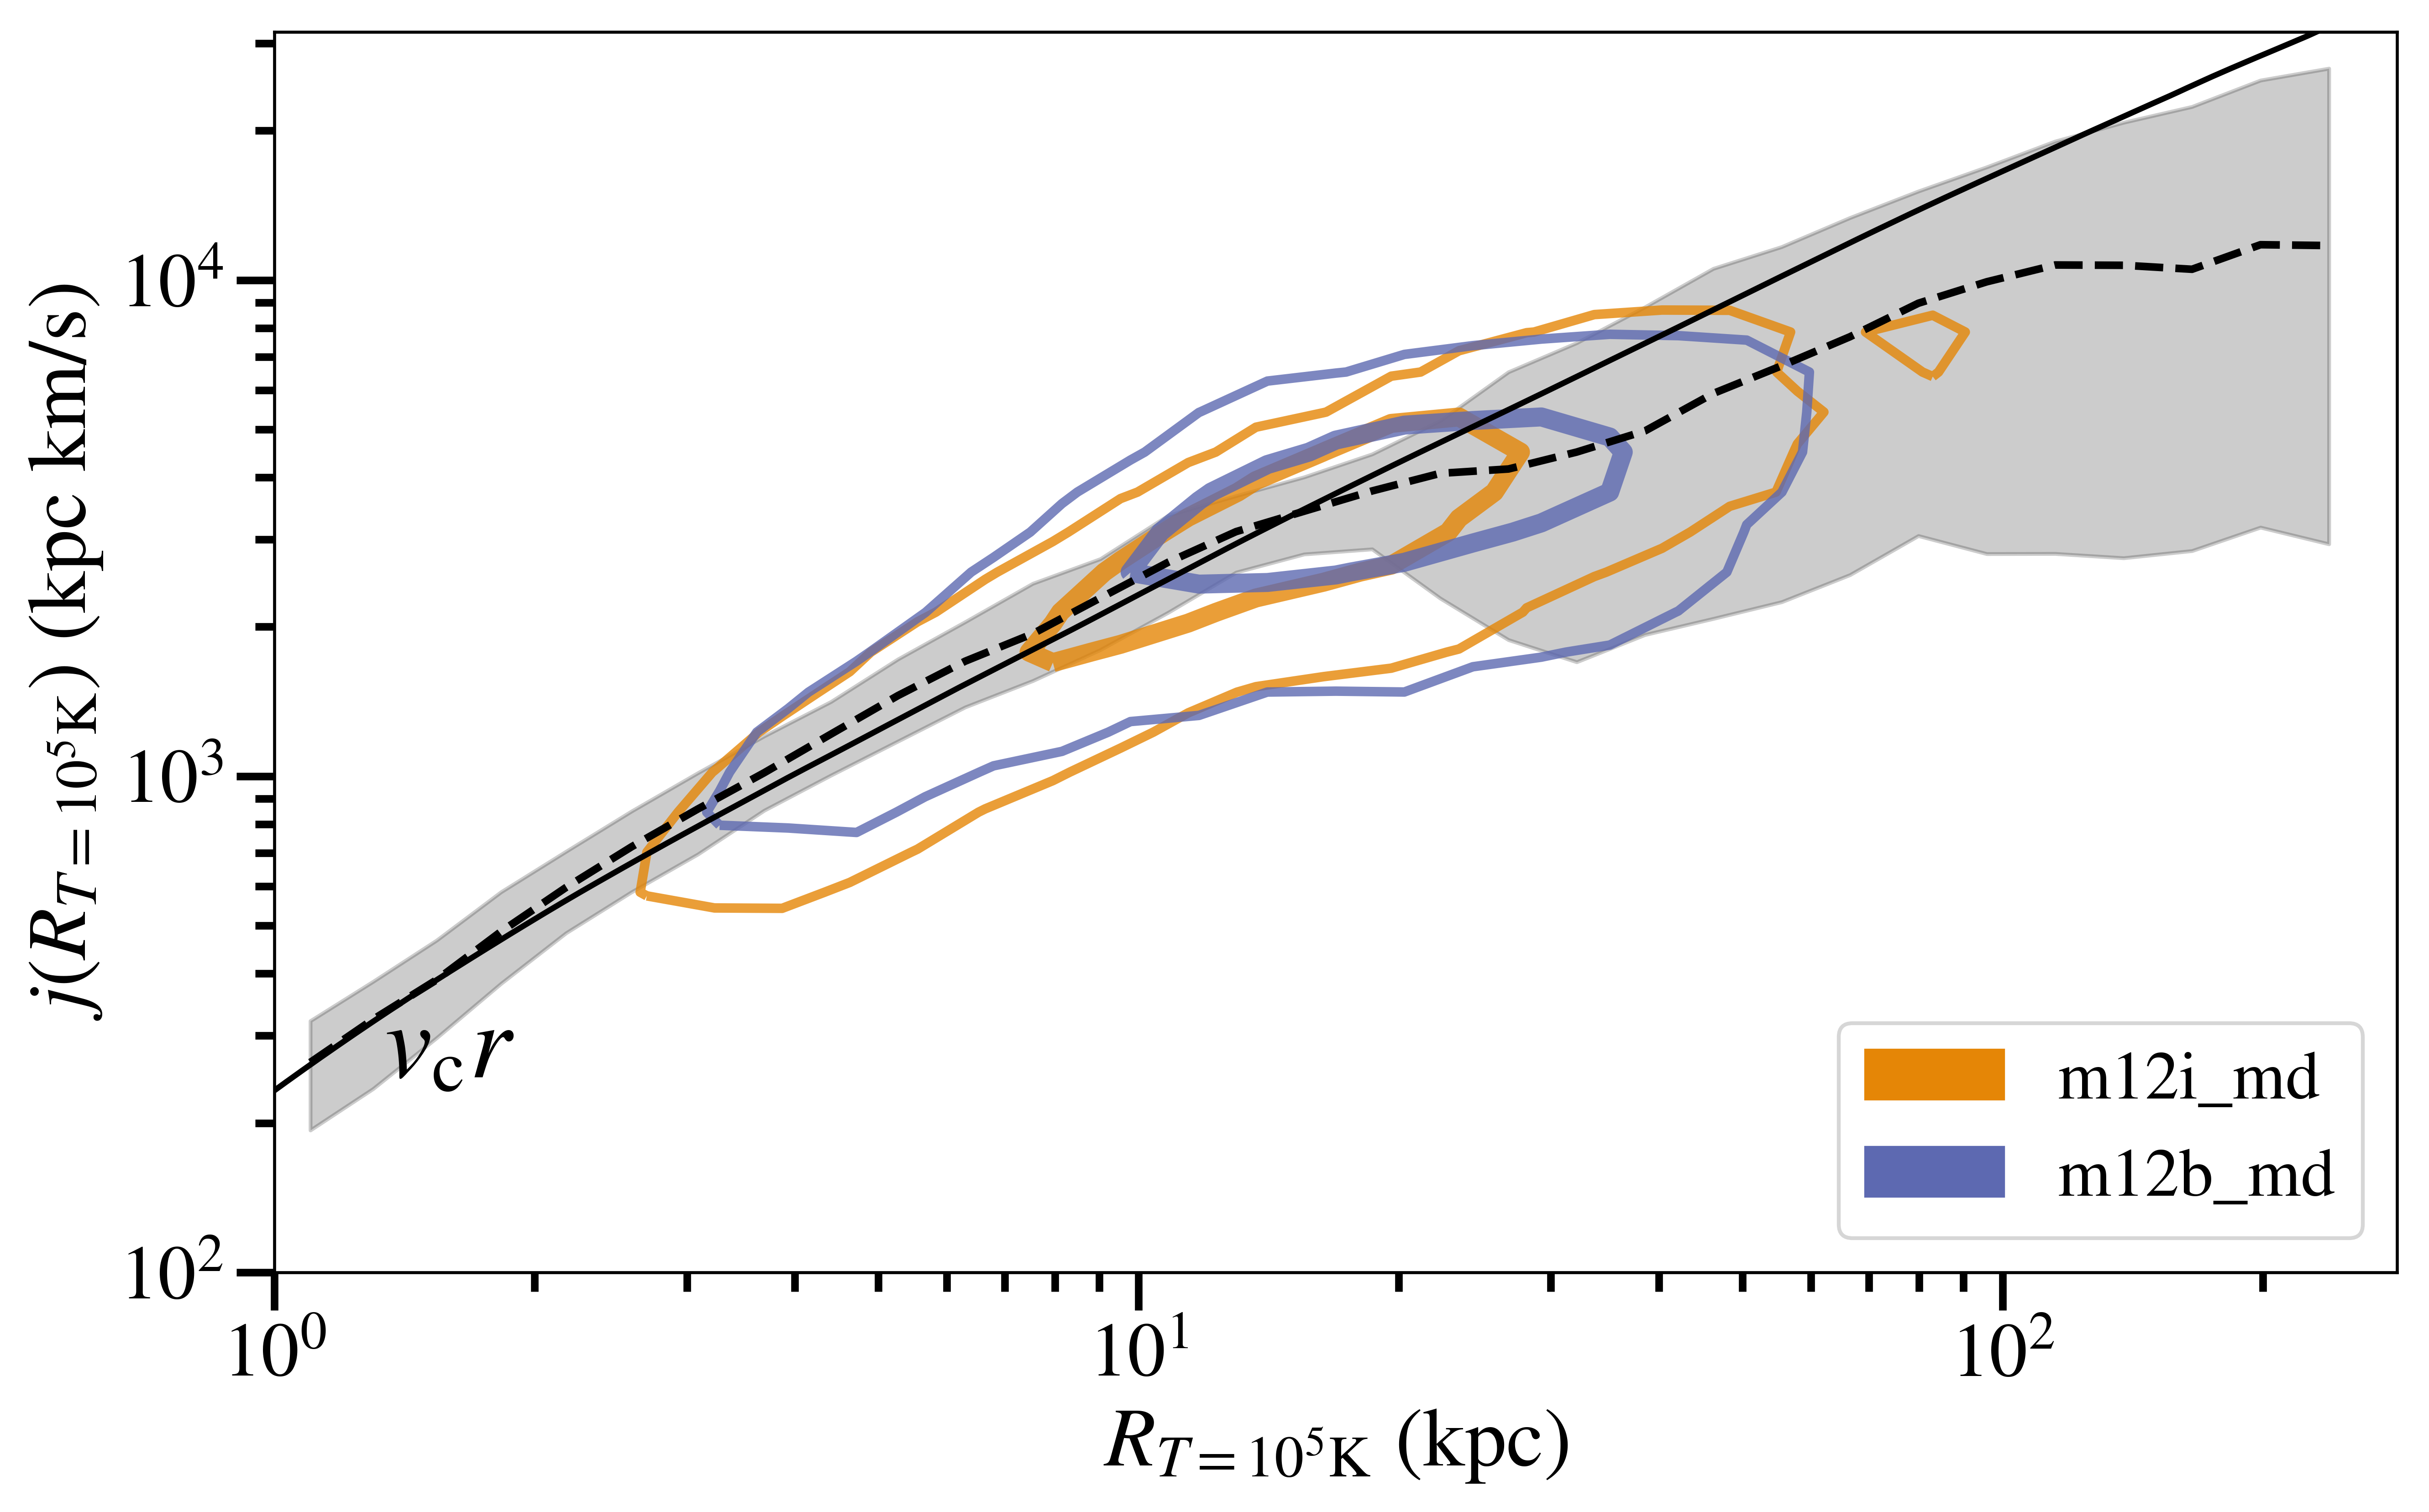
\includegraphics[width=\columnwidth]{figures/j_vs_rcondense.png}
%     \caption{
%     Distribution of $\Rcool$ vs j($\Rcool$) for four FIRE-2 halos with $L(z=0) \sim L^\star$.
% Thick (thin) contours enclose values for 50\% (90\%) of the accreted gas particles.
% The angular momentum as a function of radius for all gas in \texttt{m12i} at $z=0$ is displayed as a dashed line (the median) and shaded regions (5th-95th percentiles).
% \textbf{
% Maybe delete this figure later, because it's only relevant for simulations that have a wide distribution of $\Rcool$, which are only the artificially wide non-md runs.
% }
% \textbf{Is the 100 kpc-cooling gas related to satellite galaxies?}
% \textbf{Try changing shaded region to only hot gas instead of all gas.}
% \textbf{Try histogram of r/(j/vc) instead, to demonstrate that that decreases the spread.}
% \textit{
% In all halos the distributions are consistent with $j_{\rm c} = v_{\rm c} r$, i.e. gas cools once circularized.
% This demonstrates that the variable angular momentum of incoming gas drives the width in the $\Rcool$ distribution.
% }
%     }
%     \label{f: jcool vs Rcool}
% \end{figure}

\section{Metal diffusion vs non-metal diffusion}

\textbf{Plot of distribution $\Rcool$ for m12i and m12i\_md overlapping. Show cooling only happens at large radii in metal diffusion sims.}

%%%%%%%%%%%%%%%%%%%%%%%%%%%%%%%%%%%%%%%%%%%%%%%%%%


% Don't change these lines
\bsp	% typesetting comment
\label{lastpage}
\end{document}

% End of mnras_template.tex
